\documentclass[11pt,a4paper]{article}
\usepackage[utf8]{inputenc}
\usepackage{amsmath}
\usepackage{amsfonts}
\usepackage{amssymb}

\usepackage{graphicx}
\usepackage{float}

\usepackage[german]{babel}

\usepackage[left=3cm, right=3cm, top=3cm, bottom=3cm]{geometry}
\numberwithin{equation}{section}

\author{David Bailey}
\title{Versuchsprotokoll 2-3}

\begin{document}
\selectlanguage{german}

\begin{titlepage}
	\centering
	{Leibniz Universität Hannover\par}
	{\large Grundlagenlabor II\par}	

	\vspace{4.5cm}	
	
	{\huge \bf Versuch 2-3 \par}
	{\Huge \bf Leistung im Wechselstrom\par}
	\vspace{0.3cm}
	
	\vspace{1.5cm}
	
	{\Large David Bailey\par}

	\vfill

	\raggedright

{\Large
\begin{tabular}{ll}
Matrikelnummer:& 10011830 \\
E-Mail: & davidbailey.2889@gmail.com \\
Gruppennummer:& 218 \\
Versuch durchgeführt:& 11.12.2018 \\
Abgabe des Berichtes:& 25.12.2018
\end{tabular}\par}

\end{titlepage}


\tableofcontents

\newpage

\section{Einleitung}

Der in diesem Protokoll beschriebene Versuch \textit{Leistung bei Wechselstrom} befasst sich mit dem Problem der Leistung von periodisch bzw. harmonisch erregten Netzwerken. Es wird auf die verschiedenen Arten von Leistung sowie deren technische Relevanz eingegangen, und verschiedene Methoden der Bestimmung, Berechnung und Darstellung der Leistung werden genauer untersucht.

\subsection{Leistung bei harmonischer Erregung}

Die Grundlage der Leistungsberechnung stellt die Leistung bei harmonischer Erregung dar. Sie beschreibt für ein gegebenes lineares Netzwerk mit sinusförmigen Strömen und Spannungen die abgegebene oder aufgenommene Leistung mithilfe der komplexen Wechselstromrechnung.\\
\\
Für den Fall von $f=0$, d.h. bei einer Erregung mit Gleichstrom, ist bekannt das gilt:
\begin{align*}
P=U\cdot I
\end{align*}
\\
Liegt jedoch eine harmonische Erregung vor, so gilt der obige Term nicht mehr. Strom und Spannung sind nun zeitlich abhängig und können phasenverschoben sein, weshalb man den Zeitpunkt $t$ mit in die Formel aufnehmen muss. Es ergibt sich so der Term der \textit{Momentanleistung}:
\begin{equation} \label{eq:Momentanleistung}
p(t)=u(t)\cdot i(t)
\end{equation}
\\
Dieser gilt nun für alle Arten von Erregung und Belastung. Im Falle der harmonischen Erregung eines Verbrauchers mit den Größen:
\begin{align*}
u(t) &= \hat{U}\sin(\omega t + \varphi_u)\\
i(t) &= \hat{I}\sin(\omega t + \varphi_i)
\end{align*}
lässt sich Formel \eqref{eq:Momentanleistung} schreiben als:
\begin{eqnarray}
&p(t)=&\hat{U}\sin(\omega t + \varphi_u) \cdot \hat{I}\sin(\omega t + \varphi_i) \nonumber \\
\Leftrightarrow & p(t) =&\frac{\hat{U}\hat{I}}{2}\left[\underbrace{\cos(\varphi_u-\varphi_i)[1-\cos(2(\omega t + \varphi_u))]}_{p_w(t)}-\underbrace{\sin(\varphi_u-\varphi_i)\cdot\sin(2(\omega t + \varphi_u))}_{p_B(t)}\right] \label{eq:MomLeistungSplit}
\end{eqnarray}

Bei genauerer Betrachtung von Formel \eqref{eq:MomLeistungSplit} wird festgestellt:
\begin{enumerate}
\item Der Term der Leistung hat die doppelte Frequenz der ursprünglichen Erregung, erkennbar an $\cos(\mathbf{2\omega t} + 2\varphi_u)$ bzw. $\sin(\mathbf{2\omega t} + 2\varphi_u)$.

\item Der Durchschnitt der Leistung liegt nicht bei 0, es wird im Durschnitt eine Leistung, die sog. Wirkleistung, aufgenommen. Sie entspricht:
\begin{equation}
P = \frac{\hat{U}\hat{I}}{2}\cos(\varphi_u-\varphi_i) \label{eq:LeistungGleichanteil}
\end{equation}

\item Es gibt einen um $\frac{\pi}{2}$ zu dieser Gleichanteil-verursachenden Schwingung versetzte Leistung, welche im Durchschnitt keinen Beitrag zur aufgenommenen Leistung beiträgt. Diese als Blindleistung "Q" bezeichnete Leistung hat eine Amplitude von:
\begin{equation}
Q = \frac{\hat{U}\hat{I}}{2}\sin(\varphi_u - \varphi_i) \label{eq:LeistungBlindanteil}
\end{equation}
\end{enumerate}

Die durch Gleichung \eqref{eq:LeistungGleichanteil} angegebene Wirkleistung ist die in der Maschine tatsächlich umgesetzte elektrische Leistung, die durch Gleichung \eqref{eq:LeistungBlindanteil} angegebene Blindleistung wird periodisch von der Maschine aufgenommen und wieder abgegeben, und stellt somit einen unerwünschten Energieaustausch dar.

Die \textit{Scheinleistung} ist die Amplitude der Momentanleistung. Da Blind- und Wirkleistung exakt $\frac{\pi}{2}$ zueinander versetzt sind, lässt sie sich berechnen als:
\begin{equation}
S^2=P^2 + Q^2 = \left(\frac{\hat{U}\hat{I}}{2}\right)^2\cdot \underbrace{(\cos(\varphi_u - \varphi_i)^2 + \sin(\varphi_u - \varphi_i)^2)}_{1}
\end{equation}

Die obigen Formeln lassen sich auch mit der Komplexen Wechselstromrechnung ausdrücken. Diese kodiert den Phasenwinkel von Strom und Spannung im Argument der komplexen Zahl, während die Amplitude der Schwingungen im Betrag zu finden ist. Man kann so also auch schreiben:
\begin{equation}
\underline{S} = \underline{U}\cdot\underline{I}^* = UI\cdot e^{i(\varphi_u-\varphi_i)} \label{eq:KomplexS}
\end{equation}

Gleichungen \eqref{eq:LeistungGleichanteil} und \eqref{eq:LeistungBlindanteil} können nun auch mit der komplexen Scheinleistung ausgedrückt werden:
\begin{eqnarray*}
P=& \mbox{real}(\underline{S}) = UI\cdot \cos(\varphi_u-\varphi_i)\\
Q=& \mbox{img}(\underline{S}) = UI\cdot \sin(\varphi_u-\varphi_i)
\end{eqnarray*}

\subsection{Leistung bei periodischer Erregung}
Liegt ein lineares Netzwerk mit nicht-harmonischer Erregung vor, oder wird ein nichtlineares Bauteil verwendet, so liegen an einem Verbraucher-Zweipol keine harmonischen Ströme und Spannungen mehr an. Dementsprechend können die obigen Formeln nicht mehr angewendet werden. Insbesondere gelten Formeln \eqref{eq:LeistungGleichanteil} und \eqref{eq:LeistungBlindanteil} für Wirk- und Blindleistung nicht mehr.

Durch Verfahren wie der Fourier-Transformation der am Verbraucher gemessenen Ströme und Spannungen kann jedoch auch eine Formel der Momentanleistung berechnet werden. Setzt man die Fourier-Transformierten Ströme und Spannungen in Gleichung \eqref{eq:Momentanleistung} ein, so erhält man:
\begin{equation*}
p(t)=u(t)\cdot i(t) = \sum\sum\left(I_\nu\sin(\nu \omega t+ \varphi_{i\nu})\right) \cdot \left(U_\mu\sin(\mu \omega t + \varphi_{u\mu})\right)
\end{equation*}

Durch ähnliche trigonometrische Umformungen wie für Gleichung \eqref{eq:MomLeistungSplit} verwendet wurden, erhält man:
\begin{equation}
p_{\mu\nu}(t)=\frac{\hat{U}_\mu\hat{I}_\nu}{2}\left[\cos((\mu-\nu)\omega t + (\varphi_{u\mu}-\varphi_{i\nu}))-\cos((\mu+\nu)\omega t + (\varphi_{u\mu}-\varphi_{i\nu}))\right]
\end{equation}

Aus dieser Gleichung kann man erkennen, dass nur Oberwellen gleicher Frequenz einen Gleichanteil, und somit Wirkleistung, beitragen können. Alle anderen Kombinationen schwingen immer um 0, und tragen somit nur zur Blindleistung bei.

Die Wirkleistung eines nicht-harmonischen bzw. nichtliearen Systemes lässt sich somit berechnen als:
\begin{equation}
P_{ges}=\sum_{\mu = 1}^mP_{\mu=\nu}=\sum_{\mu = 1}^m\frac{\hat{U}_\mu\hat{I}_\mu}{2}\cos(\varphi_{u\mu}-\varphi_{i\mu})
\end{equation}

\subsection{Leistungsmessung}
Die Messung der Leistung eines elektrischen Verbrauchers ist eine in der Praxis sehr wichtige Aufgabe, so z.B. um den Stromverbrauch von Geräten zu bestimmen. Es sollen hier also zwei im späteren Versuchsverlauf genutzte Wege der (Wirk)Leistungsbestimmung genauer erläutert werden.

\subsubsection{Darstellung der Leistung}
Um die Phasenverschiebung der harmonischen Leistung bzw. die Form der periodischen Leistung bei nicht-harmonischer Erregung genauer betrachten zu können ist es oft nötig, die $p(t)$-Kurve dar zu stellen. Da fast immer mit Frequenzen von einigen zehn bis hundert Herz gearbeitet wird, lassen sich normale Multimeter nicht mehr verwenden.

Trägheitsarme Anzeigegeräte wie Logikanalysatoren oder Oszilloskope lassen sich jedoch gut verwenden, da sie analoge Signale bis zu einigen tausend Herz anzeigen können. Da sie meist nur Spannungseingänge besitzen, wird der zu messende Strom über einen möglichst geringen Widerstand geleitet, und die dort abfallende Spannung gemessen. So lässt sich die Phasenverschiebung zwischen Strom und Spannung ablesen, aber auch der genaue Verlauf bei einer nichtlinearen Belastung.

Oszilloskope besitzen zusätzlich eine Funktion zum Multiplizieren der Spannungsverläufe. So lässt sich eine zur Leistung proportionale Kurve darstellen, an der sich die doppelte Frequenz, Phasenverschiebung und der Gleichanteil ablesen lassen.

\subsubsection{Wirkleistungsmessung}
Ist nur der Betrag der Wirkleistung, nicht aber die genaue Form, Phasenverschiebung oder die Blindleistung von Interesse, so können auch träge Messgeräte, welche den Mittelwert eines hochfrequenten Signals bilden, zusammen mit einem sog. Multiplikator verwendet werden, um die in einem Verbraucher aufgenommene Wirkleistung zu bestimmen. Der Multiplikator kann hierbei entweder dem Messgerät vorgeschaltet sein, oder aber im Messgerät selbst durch mechanische Verfahren eingebaut sein.

Wird an den Eingängen des Multiplikators nun die am Verbraucher anliegende Spannung und die über einen Messwiderstand abfallende, zum Strom proportionale Spannung, angelegt, so bildet dieser nun nach Gleichung \eqref{eq:Momentanleistung} einen zur Momentanleistung proportionalen Wert. Wird dieser an ein träges Messgerät angeschlossen, so bildet dieses bei höheren Frequenzen den Durchschnitt der Momentanleistung, d.h. nach Gleichung \eqref{eq:MomLeistungSplit} einen zur Wirkleistung proportionalen Wert. Durch Bestimmung der Proportionalitätskonstante kann nun aus dem Ausschlag des Messgerätes die Wirkleistung abgelesen werden.

\subsubsection{Blindleistungsmessung}
Es lässt sich auch die Blindleistung mit einem zur Wirkleistungsmessung ähnlichem Aufbau messen. Da, angegeben von Gleichung \eqref{eq:MomLeistungSplit} die Blindleistung um $\frac{\pi}{2}$ von der Wirkleistung phasenverschoben ist, kann sie durch Phasenverschiebung der Spannung relativ zum Strom gemessen werden.
Durch Einbau eines passend gewählten Kondensators, etwa $\frac{1}{\omega C} = 10R_i$, wird diese Phasenverschiebung der gemessenen Spannung erreicht. Durch den zusätzlichen Widerstand jedoch verringert sich auch die Amplitude der gemessenen Spannung, und somit auch die der Momentanleistung. Dies muss in der Proportionalitätskonstante mit beachtet werden.

\section{Versuchsdurchführung und Auswertung}
\subsection{Messung der Momentanleistung}
\label{sec:Versuch2.2.1}
Dieser Versuchsteil befasst sich mit der grafischen Darstellung der Momentanleistung mithilfe eines Oszilloskopes. Der Verlauf von Strom und Spannung, deren Phasenverschiebung zueinander, und der Zusammenhang zum Verlauf der Momentanleistung wird betrachtet.


\subsubsection{Versuchsaufbau}
\label{sec:Aufbau2.2.1}

Abbildung \ref{fig:Plan2-1} zeigt den in diesem Versuchsteil verwendeten Schaltplan. Folgende Parameter werden verwendet:
\begin{itemize}
\item $Z_1 = \frac{1}{j\omega C} \mbox{ mit } C=4\mu F$
\item $Z_2 = 60\Omega$
\item $Z_3 = R_{sp} + j\omega L$ mit $R_{sp} = 5,5\Omega; L=15,84mH$
\item $u_{ges}$ wird durch Veränderung von $R_I$ auf 6V eingestellt.
\end{itemize}

\begin{figure}[h]
\centering
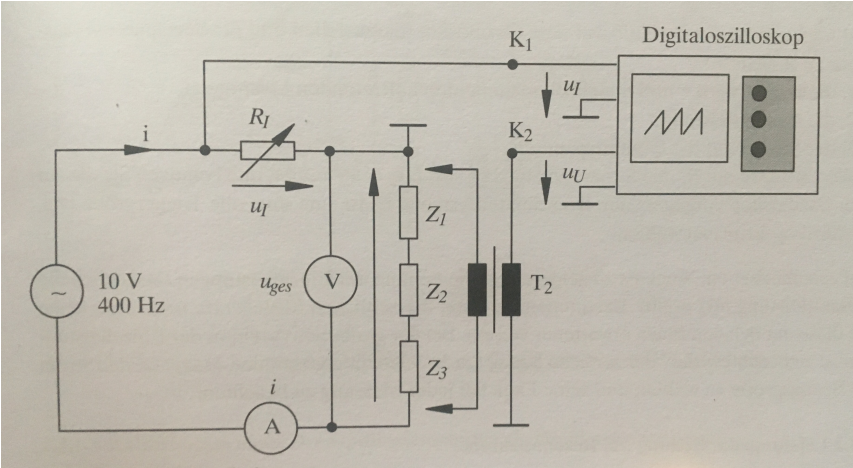
\includegraphics[width=0.7\linewidth]{Images/Aufbau2-1.png}
\caption{Schaltplan Versuch 2.1}
\label{fig:Plan2-1}
\end{figure}
\large{REFERENCE}

Im Folgenden wird das Oszilloskop zur Anzeige der Momentanleistung verwendet. Hierfür wird die Spannung über einen beliebigen Verbraucher mithilfe des potentialtrennenden Transformators $T_2$ am Oszilloskopeingang gemessen. Der Strom $i$ wird anhand der am Widerstand $R_I$ abfallenden Spannung gemessen. Zusätzlich lässt sich der Effektivwert des Stromes am Ampermeter ablesen.

Das Oszilloskop nun wird so eingestellt, dass das Produkt aus $u_I$ und $u_U$ angezeigt wird. Da $u_I$ proportional zu $i$ ist, wird so eine zur Momentanleistung proportionale Kurve angezeigt.

\subsubsection{Momentanleistungskurven}

Die im Folgenden dargestellten Kurven werden vom Oszilloskop abgespeichert. \textit{Ch~1} (blaue Kurve) stellt hierbei die zum Strom proportionale Kurve dar, \textit{Ch~2} (rote Kurve) die am Verbraucher gemessene Spannung. Die Momentanleistung $p(t)$ wird durch die grüne Kurve dargestellt.
\\
Folgende Kurven werden gemessen:

\paragraph{Momentanleistung am Kondensator}
Sie ist in Abbildung \ref{fig:MomLKurveZ1} dargestellt. Deutlich zu sehen ist die Phasenverschiebung von Strom und Spannung, welche bei ca. $\frac{\pi}{2}$ liegt. Die Kurve der Momentanleistung schwingt mit doppelter Frequenz um 0, besitzt also keinen Gleichanteil. Dies entspricht genau der Vorhersage von Gleichung \eqref{eq:MomLeistungSplit} bzw. \eqref{eq:LeistungGleichanteil}, welche für eine Phasenverschiebung von $\varphi_u - \varphi_i = -\frac{\pi}{2}$, wie sie beim Kondensator vor liegt, eine rein sinusförmige Schwingung und keine Wirkleistung vorhersagen. Der Kondensator nimmt somit entsprechend Gleichung \eqref{eq:KomplexS} eine Leistung von $\underline{S} = UIe^{-i\frac{\pi}{2}}$ auf.\par

\begin{figure}[H]
\centering
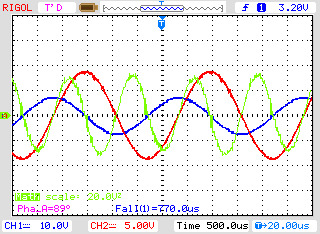
\includegraphics[width=0.7\linewidth]{Oszi-Bitmaps/NewFile0.jpg}
\caption{Momentanleistung am Kondensator. $u_I(t)$ (Blau), $u_{Z1}(t)$ (Rot), $p_{Z_1}(t)$ (Grün)}
\label{fig:MomLKurveZ1}
\end{figure}

\paragraph{Momentanleistung am Ohm'schen Widerstand}
Die Kurve der an einem Ohm'schen Widerstand gemessenen Momentanleistung ist in Abbildung \ref{fig:MomLKurveZ2} zu sehen. Da es sich um einen Verbraucher mit rein realer Impedanz handelt, gibt es keine Phasenverschiebung zwischen $u(t)$ und $i(t)$. Dies ist deutlich in der Grafik zu erkennen. Entsprechend Gleichung \eqref{eq:MomLeistungSplit} sollte die Kurve der Momentanleistung für $\varphi_u = \varphi_i$ rein positiv sein, und einen deutlichen Gleichanteil von $UI$ besitzen. Auch dies ist in der Grafik klar erkennbar. Der Widerstand nimmt also konstant Leistung auf, es wird keine Leistung abgegeben. Entsprechend Gleichungen \eqref{eq:LeistungGleichanteil} und \eqref{eq:LeistungBlindanteil} ist die Wirkleistung maximal, die Blindleistung minimal.


\begin{figure}[H]
\centering
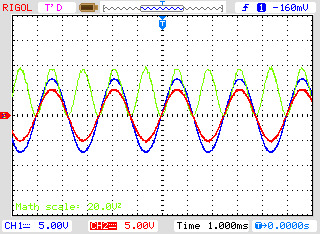
\includegraphics[width=0.7\linewidth]{Oszi-Bitmaps/NewFile1.jpg}
\caption{Momentanleistung am Ohm'schen Widerstand. $u_I(t)$ (Blau), $u_{Z2}(t)$ (Rot), $p_{Z_2}(t)$ (Grün)}
\label{fig:MomLKurveZ2}
\end{figure}

\paragraph{Momentanleistung an einer Spule}
Die Kurve der an einer Spule mit nicht-vernachlässigbarem Innenwiderstand ($R_{sp} = 5\Omega)$ ist in Abbildung \ref{fig:MomLKurveZ3} zu sehen. Ähnlich wie beim Kondensator (Abbildung \ref{fig:MomLKurveZ1}) ist eine Phasenverschiebung zwischen Strom und Spannung zu sehen. Diese ist jedoch etwas kleiner als die für eine reine Induktivität erwarteten $\frac{\pi}{2}$, welches sich durch den Innenwiderstand erklären lässt. Durch eine Komplexe Impedanz von $\underline{Z} = R_{sp} + j\omega L = 5,5\Omega + j39,81\Omega$ lässt sich eine Phasenverschiebung von $arc(\underline{Z}) = 82,134^\circ$ erwarten. Dies stimmt in etwa mit der Messung des Oszilloskopes überein. Entsprechend Gleichung \eqref{eq:MomLeistungSplit} sollte die Kurve der Momentanleistung einen kleinen Gleichanteil von etwa $P = \cos(\varphi)*S=0.136*S$ besitzen. Auch dies lässt sich in der Abbildung erkennen. Dennoch überwiegt entsprechend Gleichung \eqref{eq:LeistungBlindanteil} die Blindleistung der Spule mit $Q=\sin(\varphi)*S=0.99*S$

\begin{figure}[H]
\centering
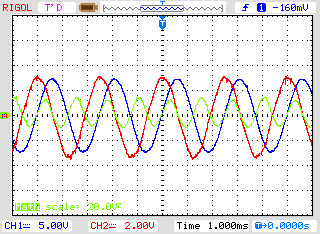
\includegraphics[width=0.7\linewidth]{Oszi-Bitmaps/NewFile2.jpg}
\caption{Momentanleistung an einer Spule mit Innenwiderstand. $u_I(t)$ (Blau), $u_{Z3}(t)$ (Rot), $p_{Z_3}(t)$ (Grün)}
\label{fig:MomLKurveZ3}
\end{figure}

\paragraph{Momentanleistung der gesamten Schaltung}
Die Kurve der in der gesamten Schaltung verbrauchten Momentanleistung ist in Abbildung \ref{fig:MomLKurveGesamt} zu erkennen. Da es sich hier um eine beliebig zusammengesetzte komplexe Impedanz handelt, lässt sich direkt keine Vorhersage über den Verlauf der Momentanleistung formulieren. Der hohe Gleichanteil legt jedoch nahe, dass die am Widerstand abfallende Leistung überwiegt. Die Phasenverschiebung lässt sich aus der Grafik als $\varphi = -\frac{\pi}{4}$ ablesen, und stimmt der obigen Vermutung zu.
Durch Summierung der Impedanzen der Komponenten lässt sich die Gesamtimpedanz berechnen:
\begin{eqnarray*}
\underline{Z}_{ges} =& \sum_{\mu=1}^3\underline{Z}_\mu = 65.5\Omega - j59.66\Omega\\
\mbox{Arg}(\underline{Z}) =& -42.33^\circ
\end{eqnarray*}
Die berechnete Phasenverschiebung entspricht hier also fast genau der anhand der Abbildung geschätzten.

Entsprechend Gleichungen \eqref{eq:LeistungGleichanteil} und \eqref{eq:LeistungBlindanteil} ist es also tatsächlich so, dass Blind- und Scheinleistung hier etwa den gleichen Betrag von $\sin(45^\circ)*S=\cos(45^\circ)*S = \frac{1}{\sqrt{2}} * S$ besitzen.

\begin{figure}[H]
\centering
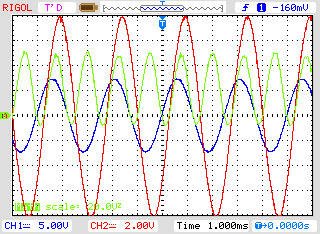
\includegraphics[width=0.7\linewidth]{Oszi-Bitmaps/NewFile3.jpg}
\caption{Momentanleistung der gesamten Schaltung. $u_I(t)$ (Blau), $u_{ges}(t)$ (Rot), $p_{ges}(t)$ (Grün)}
\label{fig:MomLKurveGesamt}
\end{figure}

\subsubsection{Grafische Addition der Leistung}
Es wird nun noch überprüft, ob sich die Momentanleistung der einzelnen Impedanzen addieren lassen, um die Momentanleistung des gesamten Systemes zu erhalten. Hierfür werden für einige beliebig gewählte Phasenwinkel die Werte der Momentanleistung aus den Oszilloskop-Messungen abgelesen, und miteinander verglichen.

\begin{center}
\begin{tabular}{| r | c | c | c | c | c|}
\hline
\multicolumn{6}{|c|}{Tabelle 1: Abgelesene Momentanleistungswerte} \\
\hline
$\varphi$ & $p_{Z_1}$ & $p_{Z_2}$ & $p_{Z_3}$  & $p_{Z_{sum}}$ & $p_{Z_{ges}}$ \\
\hline 
$0^\circ$ & $0V^2$ & $0V^2$ & $0V^2$ & $0V^2$ & $0V^2$ \\
$45^\circ$ & $-30V^2$ & $20V^2$ & $10V^2$ & $0V^2$ & $0V^2$\\
$90^\circ$ & $0V^2$ & $35V^2$ & $0V^2$ & $35V^2$ & $30V^2$ \\
\hline
\end{tabular}
\end{center}

Abgesehen von einer leichten Diskrepanz bei $\varphi = 90^\circ$ welche durch die Ungeauigkeit beim Ablesen erklärt werden kann, gleicht sich die Summe der einzelnen Momentanleistungen mit der im gesamten System verbrauchten Leistung. Dies ist auch mathematisch zu erwarten, da gilt:
\begin{eqnarray*}
& \underline{S}_{ges} =& \underline{U}_{ges}\cdot\underline{I}^* \\
\Leftrightarrow &\underline{S}_{ges} =& \underline{Z}_{ges}\cdot\underline{I}\cdot\underline{I}^* = \underline{Z}_{ges}\cdot |\underline{I}|^2 \\
\Leftrightarrow & \underline{S}_{ges} =& \underbrace{(\underline{Z}_1 + \underline{Z}_2 + \underline{Z}_3)}_{Z_{ges}} \cdot |\underline{I}|^2 \\
\Leftrightarrow & \underline{S}_{ges} =& \sum_{\mu=1}^3 \underbrace{\left(\underline{Z}_\mu \cdot |\underline{I}|^2\right)}_{S_\mu}\\
\end{eqnarray*}
\subsection{Leistung im Resonanzfall}
\subsection{Leistung einer nichtlinearen Belastung}
\subsection{Wirkleistungsbestimmung}
\subsection{Messung der Blindleistung}

\section{Zusammenfassung}

\setcounter{section}{0}
\renewcommand{\thesection}{\Alph{section}}
\section{Literaturverzeichnis}
\section{Verwendete Geräte und Tabellen}

\end{document}
